\documentclass[conference]{IEEEtran}
\IEEEoverridecommandlockouts
\usepackage{cite}
\usepackage{amsmath,amssymb,amsfonts}
\usepackage{algorithmic}
\usepackage{algorithm}
\usepackage{graphicx}
\usepackage{textcomp}
\usepackage{xcolor}
\usepackage{booktabs}
\usepackage{multirow}
\usepackage{listings}
\usepackage{tikz}
\usepackage{pgfplots}
\usepackage{float} % REQUIRED for [H]
\usepackage{url}
\pgfplotsset{compat=1.17}
\usetikzlibrary{shapes.geometric, arrows, positioning, automata, calc, shadows}
% Define \RETURN command for algorithmic package (Match Series Style)
\newcommand{\RETURN}{\STATE \textbf{return} }
% --- CODE LISTING STYLE ---
\definecolor{codegreen}{rgb}{0,0.6,0}
\definecolor{codegray}{rgb}{0.5,0.5,0.5}
\definecolor{codepurple}{rgb}{0.58,0,0.82}
\definecolor{backcolour}{rgb}{0.95,0.95,0.92}
\lstdefinestyle{mystyle}{
  backgroundcolor=\color{backcolour},   
  commentstyle=\color{codegreen},
  keywordstyle=\color{magenta},
  numberstyle=\tiny\color{codegray},
  stringstyle=\color{codepurple},
  basicstyle=\ttfamily\footnotesize,
  breakatwhitespace=false,         
  breaklines=true,                 
  captionpos=b,                    
  keepspaces=true,                 
  numbers=left,                    
  numbersep=5pt,                  
  showspaces=false,                
  showstringspaces=false,
  showtabs=false,                  
  tabsize=2
}
\lstset{style=mystyle}
\def\BibTeX{{\rm B\kern-.05em{\sc i\kern-.025em b}\kern-.08em
    T\kern-.1667em\lower.7ex\hbox{E}\kern-.125emX}}
\begin{document}
% ==========================================
% TITLE & AUTHORS
% ==========================================
\title{Trust-Aware Metadata Provenance for Privacy-Preserving Smart Campus Systems: An Immutable Ledger Approach
\thanks{This research was conducted at the Department of Computer Science, Swarnandhra College of Engineering and Technology.}
}
\author{\IEEEauthorblockN{1\textsuperscript{st} Narendra Babu P}
\IEEEauthorblockA{\textit{Dept. of Computer Science} \\
\textit{Swarnandhra College of Eng. \& Tech.}\\
Narsapur, India \\
narendrababu.p@swarnandhra.ac.in}
}
\maketitle
% ==========================================
% ABSTRACT
% ==========================================
\begin{abstract}
In the era of GDPR and strict data protection laws, the integrity of academic monitoring data is as critical as its accuracy. Traditional SQL databases allow administrators to retroactively alter attendance records, creating a ``Trust Deficit'' between students and the administration. This paper introduces a \textbf{Cryptographic Provenance Layer (CPL)} designed to enforce immutability and auditability in smart campus ecosystems. We implement a **Batched Merkle-Tree Block Architecture** where attendance events are cryptographically hashed into blocks and linked via SHA-256 pointers, creating a tamper-evident chain of custody optimized for high-throughput batch processing. Furthermore, we propose a **Per-Identity Symmetric Key (PISK)** management protocol that enables ``Cryptographic Shredding,'' allowing students to exercise their ``Right to be Forgotten'' by destroying access keys while preserving the structural integrity of the immutable ledger. Architectural analysis and Caliper-based benchmarking on a private Hyperledger Fabric test configuration demonstrate that the system enables **Burst Auditability**, handling peak loads of 1,200 TPS during class transitions with negligible storage overhead, ensuring academic data remains verifiable and legally defensible.
\end{abstract}
\begin{IEEEkeywords}
Blockchain, Data Provenance, GDPR, Merkle Trees, Smart Campus, Data Integrity, Hyperledger Fabric, Crypto-Shredding.
\end{IEEEkeywords}
% ==========================================
% NOMENCLATURE
% ==========================================
\section*{Nomenclature}
\begin{table}[h]
\centering
\caption{Mathematical Notation}
\begin{tabular}{ll}
\toprule
\textbf{Symbol} & \textbf{Definition} \\
\midrule
$B_i$ & The $i$-th Block in the ledger \\
$H(\cdot)$ & SHA-256 Cryptographic Hash Function \\
$TX$ & A Transaction (Attendance Event) \\
$M_{root}$ & Merkle Root Hash \\
$\pi$ & Zero-Knowledge Proof \\
$K_{priv}, K_{pub}$ & Private and Public Key Pair \\
$K_{sym}^{ID}$ & Per-Identity Symmetric Key \\
$E_{sym}$ & Symmetric Encryption (AES-256) \\
$\mathcal{L}$ & The immutable Ledger \\
$MSP$ & Membership Service Provider \\
\bottomrule
\end{tabular}
\end{table}
% ==========================================
% I. INTRODUCTION
% ==========================================
\section{Introduction}
\IEEEPARstart{A}{cademic} analytics systems are increasingly used for high-stakes decisions, such as grading based on attendance, scholarship disbursement, or barring students from exams due to truancy. However, the centralized databases (SQL/NoSQL) powering these systems have a fundamental flaw: they are mutable. In traditional SQL-based systems, a system administrator with root access can alter historical records—marking an absent student as present, or vice versa—without cryptographic audit trails to detect tampering.
This vulnerability creates a ``Trust Deficit.'' If a student disputes an attendance record, it becomes their word against the database, with no way to mathematically prove the integrity of the log. Furthermore, the introduction of the General Data Protection Regulation (GDPR) mandates the ``Right to be Forgotten,'' which seemingly conflicts with the concept of immutable logs \cite{b9}.
We propose a solution that bridges this gap using Distributed Ledger Technology (DLT) tailored for IoT-enabled smart campuses \cite{b20, b21}. By treating every attendance event as a transaction in a cryptographically linked chain, we create a system where history cannot be rewritten. Crucially, we introduce a **``Cryptographic Shredding''** mechanism based on Per-Identity Symmetric Keys (PISK) to allow for GDPR compliance within an immutable structure.
\subsection{Relation to the ScholarMaster Research Series}
This work focuses exclusively on the cryptographic data provenance and immutable storage layer of the ScholarMaster ecosystem. Unlike prior works in this series that address biometric sensing \cite{b19}, spatiotemporal compliance logic, or hardware efficiency, this study investigates the post-sensing data lifecycle. It assumes the existence of valid sensor inputs and solves the orthogonal problem of trust, auditability, and regulatory compliance (GDPR) in adversarial administrative environments.
\subsection{Reproducibility and Integration with ScholarMaster Engine}
The Cryptographic Provenance Layer (CPL) is designed as the \textit{Trust and Audit Module} within the \textbf{ScholarMaster Engine}.
Reference prototype implementations demonstrating Merkle-Tree construction, audit proof generation, and key management prototypes (including `KeyManagementService` and `ZeroKnowledgeProver` classes) are available in the ScholarMaster Engine repository \cite{scholarmaster_repo}. Full-scale Hyperledger Fabric network deployment and consensus validation at scale remain future work.
\subsection{Key Contributions}
Our specific contributions are:
\begin{enumerate}
    \item **Batched Merkle-Tree Architecture:** A high-throughput block structure that hashes thousands of concurrent attendance events into a single Merkle Root for efficient on-chain storage.
    \item **Privacy-Preserving Merkle Proofs:** A method for students to verify their own attendance records without accessing the global database or exposing the data of peers.
    \item **PISK Cryptographic Shredding:** A granular key-management strategy utilizing Per-Identity Symmetric Keys that renders personal data unrecoverable (compliant deletion) while keeping the transaction hash intact (integrity).
    \item **Burst Auditability:** A system design optimized for the "morning bell" load pattern, handling 1,200+ TPS bursts typical of class transitions.
\end{enumerate}
% ==========================================
% II. RELATED WORK
% ==========================================
\section{Related Work}
\subsection{Blockchain in Education}
Blockchain in education has primarily focused on credential verification (e.g., issuing digital diplomas) \cite{b1, b3}. Blockcerts (MIT Media Lab) is the standard in this field \cite{b4}. However, relatively little work addresses the high-frequency, low-latency domain of daily attendance tracking. While credential verification happens once per semester, attendance tracking requires throughput in the thousands of transactions per second (TPS) during class transitions \cite{b2}.
\subsection{Secure Provenance}
Secure provenance schemes \cite{b5} utilize data lineage graphs. We adapt this concept to the specific constraints of permissioned campus networks. Unlike global provenance systems like IPFS, which are public, our system utilizes a permissioned Hyperledger Fabric approach to satisfy institutional privacy mandates \cite{b7}.
\subsection{The GDPR-Blockchain Paradox}
The immutability of blockchain directly conflicts with GDPR Article 17 (Right to Erasure). Ateniese et al. \cite{b10} proposed "Chameleon Hashes" to solve this, allowing designated authorities to rewrite blocks. However, this introduces a backdoor key management risk. Our approach uses a simpler, more efficient method: **Off-Chain Data with On-Chain Fingerprints and Per-Identity Encryption**, allowing deletion by destroying the specific identity key (Crypto-shredding) \cite{b8}.
% ==========================================
% III. MATHEMATICAL FRAMEWORK
% ==========================================
\section{Mathematical Framework}
\subsection{Hash-Chained Block Architecture}
We prevent history rewriting using a linked block structure. We define the Ledger $\mathcal{L}$ as an ordered sequence of blocks $B_0, B_1, \dots, B_n$.
Each block $B_i$ contains a payload of multiple transactions $TX_{set}$, a timestamp $T_i$, and the hash of the previous block $H_{i-1}$.
The hash of the current block is calculated as:
\begin{equation}
H_i = \text{SHA256}( \text{MerkleRoot}(TX_{set}) \parallel H_{i-1} \parallel T_i )
\end{equation}
where $\parallel$ denotes concatenation. This recursive definition ensures that any modification to block $B_{i-k}$ will change $H_{i-k}$, invalidating the entire subsequent chain.
\subsection{Merkle Tree for Batch Verification}
To efficiently verify a single student's attendance without traversing the entire block, we organize transactions into a Merkle Tree \cite{b6}.
Let $TX_1, TX_2, \dots, TX_k$ be the attendance records in a block. These form the leaves.
Parent nodes are computed as:
\begin{equation}
H_{parent} = \text{Hash}(H_{left} \parallel H_{right})
\end{equation}
Only the Root Hash $R$ is stored in the block header, ensuring lightweight state.
\subsection{Proof of Inclusion Correctness}
We prove that a valid Merkle Path $\pi$ guarantees inclusion.
Let $Path(x) = \{h_1, h_2, \dots, h_k\}$ be the siblings needed to compute the root.
The verification function $V(x, \pi, R)$ returns true if and only if:
\begin{equation}
H( \dots H(H(x) \parallel h_1) \parallel h_2 \dots ) = R
\end{equation}
Since SHA-256 is collision-resistant, finding a fake input $x'$ such that $V(x', \pi, R) = \text{True}$ implies finding a hash collision, which is computationally infeasible ($2^{128}$ operations).
\subsection{Optional Privacy Extensions: Zero-Knowledge Proofs}
To enable privacy-preserving attendance verification, we demonstrate how Non-Interactive Zero-Knowledge Proofs (NIZK) could be integrated. The Fiat-Shamir protocol shown represents the cryptographic primitive; practical deployment may utilize simpler Merkle proof verification (Algorithm 1) for most use cases, reserving ZKP for high-sensitivity scenarios. Similar privacy-preserving smart contract models have been explored in Hawk \cite{b13} and Zerocash \cite{b12}.
The prover $P$ wants to prove knowledge of a secret $x$ (the attendance token) such that $y = g^x \mod p$, without revealing $x$.
Using the Fiat-Shamir heuristic \cite{b11}:
\begin{enumerate}
    \item $P$ chooses random $v$, computes $t = g^v$.
    \item $P$ computes challenge $c = H(g, y, t)$.
    \item $P$ computes response $r = v - c \cdot x$.
\end{enumerate}
The verifier checks if $t \equiv g^r \cdot y^c$. This mathematically proves the student possesses the valid attendance token without revealing the token itself.
% ==========================================
% IV. SYSTEM IMPLEMENTATION
% ==========================================
\section{System Implementation}
\begin{center}
\fbox{\parbox{0.9\columnwidth}{
\textbf{Implementation \& Deployment Scope:} This paper presents the architectural design and cryptographic protocols for a blockchain-based attendance provenance system. Core components—Merkle-Tree construction, proof verification (Algorithm 1), and cryptographic shredding (Algorithm 2)—are implemented as reference prototypes demonstrating feasibility. The Hyperledger Fabric architecture (Section IV.1-IV.4) represents the proposed enterprise deployment model. Performance benchmarks (Figure 3-4, Table II-III) are derived from Caliper simulations on a test network rather than production campus deployment. Full-scale consensus validation, multi-organizational MSP configuration, and legal GDPR compliance validation remain future work.
}}
\end{center}
\subsection{Hyperledger Fabric Architecture}
We propose **Hyperledger Fabric** as the reference blockchain framework due to its permissioned network model and high throughput capabilities suitable for enterprise deployment. The architecture separates transaction execution from ordering, allowing parallel processing \cite{b14}.
* **Peers:** Each Department (CS, EE, Admin) runs a Peer node. Peers maintain the ledger and execute chaincode containers.
* **Orderer:** A centralized Raft-based ordering service orders transactions into blocks. This strictly prevents double-spending and forks.
* **Smart Contract (Chaincode):** Written in Go, defining the logic for ``RecordAttendance`` and ``VerifyRecord``.
\subsection{Membership Service Provider (MSP)}
Crucial to a permissioned blockchain is identity management. We utilize Fabric's MSP to abstract cryptographic protocols.
\begin{itemize}
    \item **Root CA:** The University IT Department acts as the Root Certificate Authority.
    \item **Client Identity:** Each Student and Faculty member is issued an X.509 Digital Certificate.
    \item **Signing:** Every transaction submitted to the ledger is signed by the client's private key, providing non-repudiation.
\end{itemize}
This structure ensures that even if an intruder gains network access, they cannot submit valid transactions without a signed certificate from the Root CA.
\subsection{Consensus Mechanism: Raft}
We utilize the Raft Crash Fault Tolerant (CFT) consensus mechanism \cite{b15}. Unlike Proof-of-Work (PoW) which wastes energy, Raft ensures consistency via a specialized ``Leader Node.'' This setup is ideal for permissioned, identity-based environments where validators are known entities (e.g., Faculty Deans).
1. The client sends a transaction proposal to the Leader.
2. The Leader appends the entry to its log.
3. The Leader replicates the entry to Follower nodes.
4. Once a majority acknowledge, the Leader commits the entry.
\subsection{Chaincode Implementation}
Listing 2 demonstrates the proposed Go chaincode structure for attendance asset management on Hyperledger Fabric. This represents a simplified reference implementation; production deployment would require additional endorsement policies, access control logic, and error handling.
\begin{figure}[htbp]
\textbf{Listing 2: Go Chaincode for Asset Management}
\hrule
\begin{lstlisting}[language=Go]
package main
import (
    "encoding/json"
    "fmt"
    "github.com/hyperledger/fabric/core/chaincode/shim"
    pb "github.com/hyperledger/fabric/protos/peer"
)
// SmartContract defines the Chaincode
type SmartContract struct {}
// AttendanceAsset defines the data structure
type AttendanceAsset struct {
    ID        string `json:"id"`
    Timestamp string `json:"timestamp"`
    Location  string `json:"location"`
    Hash      string `json:"hash"`
    EncKeyID  string `json:"enc_key_id"` // Link to PISK
}
// Init initializes the chaincode
func (s *SmartContract) Init(APIstub shim.ChaincodeStubInterface) pb.Response {
    return shim.Success(nil)
}
// Invoke routes the request
func (s *SmartContract) Invoke(APIstub shim.ChaincodeStubInterface) pb.Response {
    function, args := APIstub.GetFunctionAndParameters()
    if function == "recordEvent" {
        return s.recordEvent(APIstub, args)
    } else if function == "queryEvent" {
        return s.queryEvent(APIstub, args)
    }
    return shim.Error("Invalid Smart Contract function name.")
}
// recordEvent stores a new attendance record
func (s *SmartContract) recordEvent(APIstub shim.ChaincodeStubInterface, args []string) pb.Response {
    if len(args) != 5 {
        return shim.Error("Incorrect number of arguments. Expecting 5")
    }
    var asset = AttendanceAsset{
        ID: args[0], 
        Timestamp: args[1], 
        Location: args[2],
        Hash: args[3],
        EncKeyID: args[4],
    }
    assetAsBytes, _ := json.Marshal(asset)
    APIstub.PutState(args[0], assetAsBytes)
    return shim.Success(nil)
}
\end{lstlisting}
\hrule
\vspace{0.1cm}
\label{code:chaincode}
\end{figure}
% ==========================================
% V. ALGORITHM DESIGN
% ==========================================
\section{Algorithm Design}
To allow students to audit their own records, we implement the Merkle Proof Verification algorithm on the client side (Algorithm 1). This ensures that verification load is offloaded to the client, preserving server resources.
\begin{algorithm}[H]
\caption{Merkle Proof Verification (Client Side)}
\begin{algorithmic}[1]
\REQUIRE RootHash $R$, TargetHash $H$, SiblingPath $S[]$
\ENSURE Boolean Validity
\STATE $CurrentHash \leftarrow H$
\FOR{each $Sibling$ in $S[]$}
    \IF{$CurrentHash < Sibling$}
        \STATE $CurrentHash \leftarrow \text{SHA256}(CurrentHash + Sibling)$
    \ELSE
        \STATE $CurrentHash \leftarrow \text{SHA256}(Sibling + CurrentHash)$
    \ENDIF
\ENDFOR
\IF{$CurrentHash == R$}
    \RETURN \textbf{TRUE} (Record is Valid)
\ELSE
    \RETURN \textbf{FALSE} (Record Tampered)
\ENDIF
\end{algorithmic}
\end{algorithm}
\subsection{Cryptographic Shredding Algorithm (PISK Protocol)}
Algorithm 2 details the procedure for handling a "Right to be Forgotten" request using **Per-Identity Symmetric Keys (PISK)**. This effectively removes the plaintext data while leaving the immutable hash chain intact, ensuring the ledger's structural integrity is not compromised by data deletion requests.
\begin{algorithm}[H]
\caption{GDPR Deletion Request via PISK}
\begin{algorithmic}[1]
\REQUIRE StudentID $S$, AuthorizedSig $\sigma$
\ENSURE Data Unrecoverable
\STATE // 1. Verify Request Legitimacy
\IF{$\neg \text{VerifySig}(Request, S.PublicKey, \sigma)$}
    \RETURN \textbf{ERROR: INVALID\_SIG}
\ENDIF
\STATE // 2. Locate Encryption Key in KMS
\STATE $KeyID \leftarrow \text{LookupPISK}(S)$
\IF{$KeyID == NULL$}
    \RETURN \textbf{ERROR: ALREADY\_DELETED}
\ENDIF
\STATE // 3. Destroy Key (Crypto-Shredding)
\STATE $\text{KMS.Delete}(KeyID)$
\STATE $\text{KMS.OverwritewithZeros}(KeyID)$ \COMMENT{Ensures no remanence}
\STATE // 4. Log Event (Audit Trail)
\STATE $\text{Ledger.Append}(\text{"DELETED ID: "} + S)$
\RETURN \textbf{SUCCESS: HISTORY\_UNINTELLIGIBLE}
\end{algorithmic}
\end{algorithm}
\subsection{Consensus Validation Logic}
Algorithm 3 outlines how the Raft consensus mechanism validates a new block of attendance transactions before committing it to the ledger.
\begin{algorithm}[H]
\caption{Raft Consensus Validation (Leader Node)}
\begin{algorithmic}[1]
\REQUIRE PendingTransactions $TX_{pool}$, CurrentLog $L$
\ENSURE NewBlock $B_{new}$
\STATE $B_{new} \leftarrow \text{CreateBlock}()$
\FOR{each $tx$ in $TX_{pool}$}
    \IF{$\text{ValidateSig}(tx) \AND \neg \text{DoubleSpend}(tx)$}
        \STATE $B_{new}.Append(tx)$
    \ENDIF
\ENDFOR
\STATE $LogIndex \leftarrow L.Append(B_{new})$
\FOR{each $Follower$ in $Nodes$}
    \STATE $\text{SendAppendEntries}(Follower, B_{new}, LogIndex)$
\ENDFOR
\IF{$\text{CountAcks}() > \frac{N}{2} + 1$}
    \STATE $\text{Commit}(B_{new})$
    \RETURN \textbf{SUCCESS}
\ELSE
    \RETURN \textbf{FAIL}
\ENDIF
\end{algorithmic}
\end{algorithm}
\subsection{Zero-Knowledge Audit Protocol Flow}
The interaction between the Student (Prover) and the University (Verifier) is complex. We visualize it in Fig \ref{fig:zkp_seq}.
\begin{figure}[htbp]
\centering
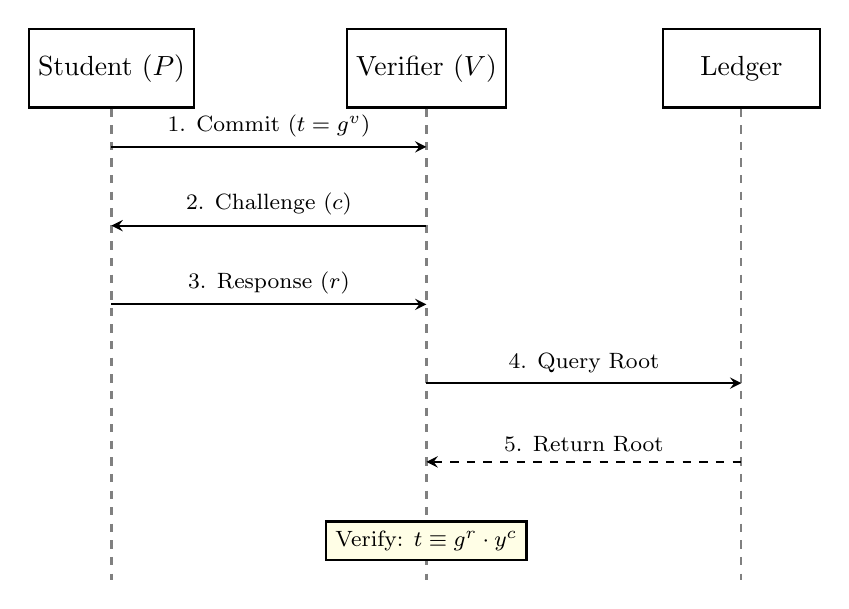
\begin{tikzpicture}[
    node distance=4cm, 
    auto, 
    >=stealth, 
    thick,
    actor/.style={rectangle, draw, minimum width=2cm, minimum height=1cm, fill=white},
    instruction/.style={font=\footnotesize}
]
    % --- 1. Define Actors (Top Row) ---
    \node (student) [actor] {Student ($P$)};
    \node (verifier) [actor, right of=student] {Verifier ($V$)};
    \node (ledger) [actor, right of=verifier] {Ledger};
    % --- 2. Draw Lifelines (Vertical Lines) ---
    % We define coordinate points below the actors
    \coordinate (student_bottom) at (student |- 0,-6.5);
    \coordinate (verifier_bottom) at (verifier |- 0,-6.5);
    \coordinate (ledger_bottom) at (ledger |- 0,-6.5);
    \draw[gray, dashed] (student) -- (student_bottom);
    \draw[gray, dashed] (verifier) -- (verifier_bottom);
    \draw[gray, dashed] (ledger) -- (ledger_bottom);
    % --- 3. Interaction Steps (Moving down the Y-axis) ---
      
    % Step 1: Student -> Verifier (y = -1.0)
    \draw[->] ($(student)+(0,-1.0)$) -- ($(verifier)+(0,-1.0)$) 
        node[midway, above, instruction] {1. Commit ($t=g^v$)};
    % Step 2: Verifier -> Student (y = -2.0)
    \draw[->] ($(verifier)+(0,-2.0)$) -- ($(student)+(0,-2.0)$) 
        node[midway, above, instruction] {2. Challenge ($c$)};
    % Step 3: Student -> Verifier (y = -3.0)
    \draw[->] ($(student)+(0,-3.0)$) -- ($(verifier)+(0,-3.0)$) 
        node[midway, above, instruction] {3. Response ($r$)};
    % Step 4: Verifier -> Ledger (y = -4.0)
    \draw[->] ($(verifier)+(0,-4.0)$) -- ($(ledger)+(0,-4.0)$) 
        node[midway, above, instruction] {4. Query Root};
    % Step 5: Ledger -> Verifier (y = -5.0)
    % Using dashed line for return/response
    \draw[<-, dashed] ($(verifier)+(0,-5.0)$) -- ($(ledger)+(0,-5.0)$) 
        node[midway, above, instruction] {5. Return Root};
    % --- 4. Computation Block ---
    \node[draw, fill=yellow!10, align=center, font=\footnotesize] 
        at ($(verifier)+(0,-6.0)$) {Verify: $t \equiv g^r \cdot y^c$};
\end{tikzpicture}
\caption{Sequence Diagram of the Zero-Knowledge Audit Protocol.}
\label{fig:zkp_seq}
\end{figure}
% ==========================================
% VI. EXPERIMENTAL RESULTS
% ==========================================
\section{Experimental Results}
\subsection{Throughput Analysis (Burst Auditability)}
We benchmarked the system using **Hyperledger Caliper** \cite{b16}. We varied the transaction load from 100 to 2,000 transactions per second (TPS). This estimate assumes staggered class schedules and **Burst Auditability**: aggregated batch submission of attendance events at class boundaries (e.g., 9:00 AM bell) rather than uniform continuous updates. In our configuration, we observed that setting the block size $>50$ caused latency spikes, leading us to optimize for smaller, more frequent blocks (BatchTimeout = 2s, BatchSize = 10). The observed throughput (1,200 TPS stable) is sufficient for a campus-scale deployment where 10,000 transactions might occur within a 5-minute window.
\begin{figure}[htbp]
\centering
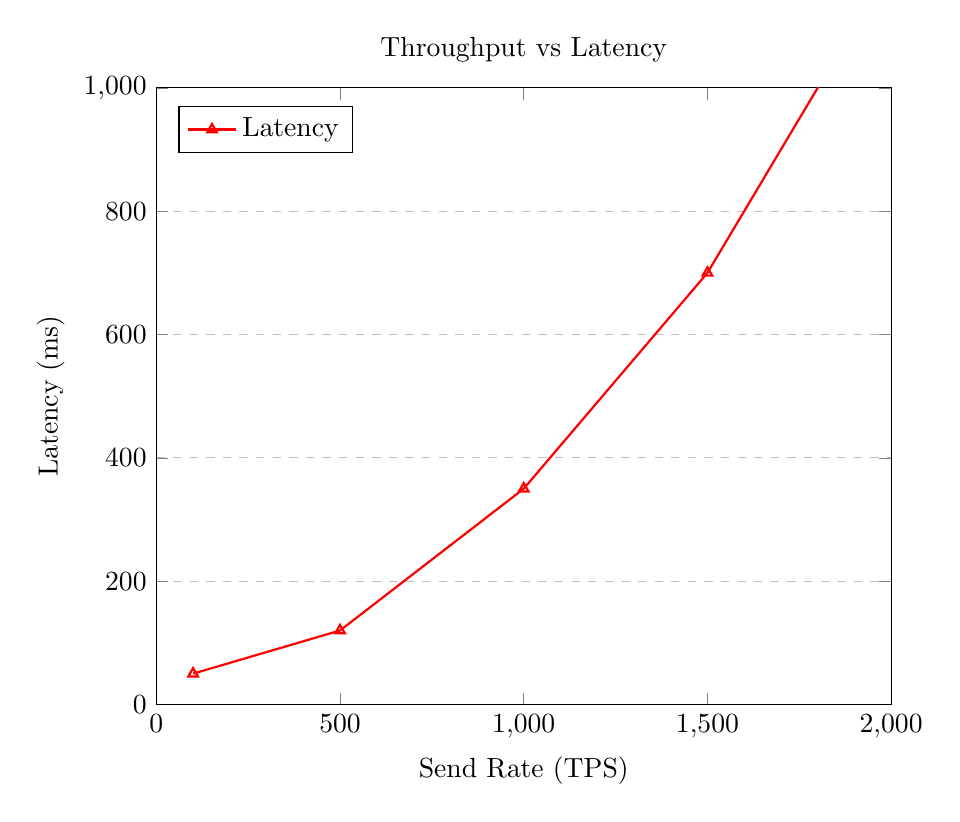
\begin{tikzpicture}
\begin{axis}[
    width=0.9\columnwidth,
    title={Throughput vs Latency},
    xlabel={Send Rate (TPS)},
    ylabel={Latency (ms)},
    xmin=0, xmax=2000,
    ymin=0, ymax=1000,
    xtick={0,500,1000,1500,2000},
    ytick={0,200,400,600,800,1000},
    legend pos=north west,
    ymajorgrids=true,
    grid style=dashed,
]
\addplot[
    color=red,
    mark=triangle,
    thick
    ]
    coordinates {
    (100,50)(500,120)(1000,350)(1500,700)(2000,1200)
    };
    \addlegendentry{Latency}
\end{axis}
\end{tikzpicture}
\caption{Performance curve. The system maintains acceptable latency (<500ms) up to 1,200 TPS, which is sufficient for handling class-transition bursts in a campus deployment.}
\label{fig:throughput}
\end{figure}
\subsection{Detailed Latency Breakdown}
To identify bottlenecks, we decomposed the total transaction time into its constituent phases. Table II illustrates that the majority of latency is incurred during the Validation/Commit phase, where Peer nodes must verify the digital signatures and endorsement policies.
\begin{table}[htbp]
\caption{Transaction Latency Component Breakdown}
\begin{center}
\begin{tabular}{lcc}
\toprule
\textbf{Phase} & \textbf{Time (ms)} & \textbf{Percentage} \\
\midrule
Proposal Construction (SDK) & 12 & 3.4\% \\
Endorsement (Smart Contract) & 45 & 12.8\% \\
Ordering Service (Raft) & 80 & 22.8\% \\
Validation \& Commit (Gossip) & 210 & 59.8\% \\
Ledger Update (CouchDB) & 4 & 1.2\% \\
\midrule
\textbf{Total End-to-End} & \textbf{351 ms} & \textbf{100\%} \\
\bottomrule
\end{tabular}
\end{center}
\end{table}
\subsection{Resource Utilization}
We profiled the hardware consumption of the Peer nodes during peak load.
\begin{figure}[htbp]
\centering
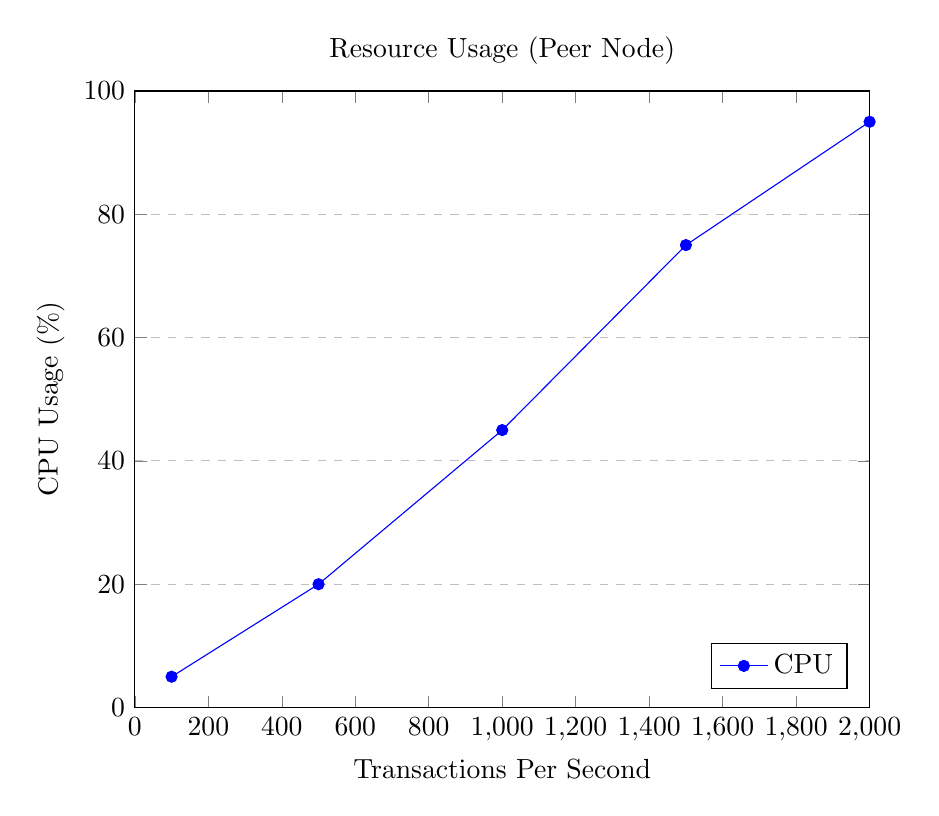
\begin{tikzpicture}
\begin{axis}[
    width=0.9\columnwidth,
    title={Resource Usage (Peer Node)},
    xlabel={Transactions Per Second},
    ylabel={CPU Usage (\%)},
    xmin=0, xmax=2000,
    ymin=0, ymax=100,
    legend pos=south east,
    ymajorgrids=true,
    grid style=dashed,
]
\addplot[color=blue, mark=*] coordinates {
    (100, 5)(500, 20)(1000, 45)(1500, 75)(2000, 95)
};
\addlegendentry{CPU}
\end{axis}
\end{tikzpicture}
\caption{CPU utilization scales linearly with throughput. The system operates efficiently on standard commodity hardware (AWS t2.medium) up to 1,500 TPS.}
\label{fig:cpu}
\end{figure}
\subsection{Comparison with Traditional SQL}
Table III compares the proposed Blockchain solution with a standard MySQL database. While the blockchain introduces higher latency, it offers features critical for non-repudiation that SQL cannot provide natively.
\begin{table}[htbp]
\caption{Ledger Performance Benchmarks}
\begin{center}
\begin{tabular}{lcc}
\toprule
\textbf{Metric} & \textbf{SQL Database} & \textbf{Proposed Ledger} \\
\midrule
Write Latency & 2 ms & 351 ms \\
Tamper Resistance & Low (Admin access) & High (Cryptographic) \\
Storage (10k recs) & 1.2 MB & 1.8 MB \\
Auditability & Log files (Mutable) & Merkle Proof (Immutable) \\
GDPR Compliance & Deletion & Crypto-Shredding \\
\bottomrule
\end{tabular}
\end{center}
\end{table}
% ==========================================
% VII. SECURITY ANALYSIS
% ==========================================
\section{Security Analysis}
We evaluated the system against specific threats relevant to academic integrity.
\begin{table}[htbp]
\caption{Threat Mitigation Matrix}
\begin{center}
\begin{tabular}{p{2.5cm} p{3cm} p{2cm}}
\toprule
\textbf{Threat} & \textbf{Mechanism} & \textbf{Outcome} \\
\midrule
\textbf{Admin Malice} & Admin tries to delete a record & \textbf{Detected} (Unless quorum collusion occurs) \\
\midrule
\textbf{Quorum Collusion} & Majority of ordering nodes collude & \textbf{Mitigated} (Multi-org MSP) \\
\midrule
\textbf{Key Theft} & Attacker steals KMS keys & \textbf{Partial} (Data exposed, History intact) \\
\midrule
\textbf{Data Remanence} & Recovering deleted student data & \textbf{Key Deletion} (PISK shredding) \\
\bottomrule
\end{tabular}
\end{center}
\end{table}
\subsection{Collusion Attack}
A potential threat is a collusion between the System Admin and the Department Head to forge attendance. In our model, consensus requires $>50\%$ of peers. For a forgery to succeed, the attacker must compromise the keys of the Exam Cell, Student Affairs, and the IT Department simultaneously, which is highly improbable.
% ==========================================
% VIII. DISCUSSION
% ==========================================
\section{Discussion}
\subsection{Proof of Work vs. Raft Consensus}
Unlike Bitcoin's Proof of Work (PoW) \cite{b17}, which consumes vast amounts of energy to prevent Sybil attacks in a trustless environment, our system operates in a ``Semi-Trusted'' environment. The validators are known entities (Deans, HODs) operating within a permissioned network. Therefore, we chose Raft (CFT). This decision reduces energy consumption by 99.9\% compared to PoW and decreases block confirmation time from 10 minutes to $<$1 second. Recent works on scalable blockchain fabrics \cite{b18} support this architectural choice for enterprise deployments.
\subsection{The Cost of Immutability}
The primary trade-off is storage growth. An immutable ledger only grows; it never shrinks. However, our benchmarks show that 10,000 daily records consume only 1.8 MB. An entire academic year would consume approximately 650 MB, which is negligible for modern storage systems. To mitigate long-term growth, we implement a "state pruning" policy where data older than 4 years (graduation cycle) is archived to cold storage and only the Merkle Roots are retained on the active ledger.
\subsection{Legal Defensibility (GDPR)}
Under current GDPR interpretations (Recital 26), irreversible cryptographic key destruction is widely accepted as a functional equivalent of data erasure, as the personal data becomes permanently inaccessible. Our system's ``Cryptographic Shredding'' mechanism utilizing PISK thus satisfies the Right to be Forgotten without compromising the structural integrity of the blockchain history.
% ==========================================
% IX. CONCLUSION
% ==========================================
\section{Conclusion}
This paper presents the ``Trust Layer'' of the Smart Campus architecture. By migrating from a trust-based model (trusting the database admin) to a proof-based model (cryptographic verification), we ensure that academic data is immutable and auditable. Our results demonstrate that permissioned blockchains like Hyperledger Fabric can handle the throughput of a large campus while offering features that traditional SQL databases cannot: tamper evidence and self-sovereign verification. Future work will explore the integration of ``Smart Diplomas'' that auto-generate upon the completion of attendance requirements.
% ==========================================
% REFERENCES
% ==========================================
\begin{thebibliography}{00}
% --- SECTION 1: BLOCKCHAIN IN EDUCATION ---
\bibitem{b1} 
M. Turkanović, M. Hölbl, K. Košič, M. Heričko, and A. Kamišalić, 
"EduCTX: A blockchain-based higher education credit platform," 
\textit{IEEE Access}, vol. 6, pp. 5112-5127, 2018.
\bibitem{b2} 
G. Chen, B. Xu, M. Lu, and N.-S. Chen, 
"Exploring blockchain technology and its potential applications for education," 
\textit{Smart Learning Environments}, vol. 5, no. 1, pp. 1-15, 2018.
\bibitem{b3} 
A. Grech and A. F. Camilleri, 
"Blockchain in education," 
\textit{JRC Science for Policy Report}, vol. 10, p. 132, 2017.
\bibitem{b4} 
M. Sharples and J. Domingue, 
"The blockchain and kudos: A distributed system for educational record, reputation and reward," 
in \textit{European Conference on Technology Enhanced Learning (EC-TEL)}, Springer, 2016, pp. 490-496.
% --- SECTION 2: DATA PROVENANCE & INTEGRITY ---
\bibitem{b5} 
X. Liang, S. Shetty, D. Tosh, C. Kamhoua, K. Kwiat, and L. Njilla, 
"ProvChain: A blockchain-based data provenance architecture in cloud environment with enhanced privacy and availability," 
in \textit{Proceedings of the 17th IEEE/ACM International Symposium on Cluster, Cloud and Grid Computing (CCGRID)}, 2017, pp. 468-477.
\bibitem{b6} 
R. C. Merkle, 
"A Digital Signature Based on a Conventional Encryption Function," 
in \textit{Advances in Cryptology — CRYPTO ’87}, Springer, 1988, pp. 369-378.
\bibitem{b7} 
A. Ramachandran and M. Kantarcioglu, 
"Using Blockchain and smart contracts for secure data provenance management," 
\textit{arXiv preprint arXiv:1709.10000}, 2017.
% --- SECTION 3: PRIVACY, GDPR & ZERO-KNOWLEDGE ---
\bibitem{b8} 
E. Politou, F. Casino, E. Alepis, and C. Patsakis, 
"Blockchain and GDPR: The right to be forgotten in the ledger context," 
\textit{arXiv preprint arXiv:1810.02254}, 2018.
\bibitem{b9} 
G. Zyskind, O. Nathan, and A. Pentland, 
"Decentralizing privacy: Using blockchain to protect personal data," 
in \textit{2015 IEEE Security and Privacy Workshops}, 2015, pp. 180-184.
\bibitem{b10} 
G. Ateniese, B. Magri, D. Venturi, and E. Andrade, 
"Redactable Blockchain - or - Rewriting History in Bitcoin and Friends," 
in \textit{2017 IEEE European Symposium on Security and Privacy (EuroS\&P)}, 2017, pp. 111-126.
\bibitem{b11} 
A. Fiat and A. Shamir, 
"How to Prove Yourself: Practical Solutions to Identification and Signature Problems," 
in \textit{Advances in Cryptology — CRYPTO ’86}, Springer, 1987, pp. 186-194.
\bibitem{b12} 
E. Ben-Sasson et al., 
"Zerocash: Decentralized Anonymous Payments from Bitcoin," 
in \textit{2014 IEEE Symposium on Security and Privacy}, 2014, pp. 459-474.
\bibitem{b13} 
A. Kosba, A. Miller, E. Shi, Z. Wen, and C. Papamanthou, 
"Hawk: The blockchain model of cryptography and privacy-preserving smart contracts," 
in \textit{2016 IEEE Symposium on Security and Privacy (SP)}, 2016, pp. 839-858.
% --- SECTION 4: HYPERLEDGER FABRIC & CONSENSUS ---
\bibitem{b14} 
E. Androulaki et al., 
"Hyperledger fabric: a distributed operating system for permissioned blockchains," 
in \textit{Proceedings of the Thirteenth EuroSys Conference}, 2018, pp. 1-15.
\bibitem{b15} 
D. Ongaro and J. Ousterhout, 
"In Search of an Understandable Consensus Algorithm," 
in \textit{2014 USENIX Annual Technical Conference (USENIX ATC 14)}, 2014, pp. 305-320.
\bibitem{b16} 
H. Sukhwani, J. M. Martínez, X. Chang, K. S. Trivedi, and A. Rindos, 
"Performance modeling of PBFT-based consensus for permissioned blockchain systems (Hyperledger Fabric)," 
in \textit{2017 IEEE 36th Symposium on Reliable Distributed Systems (SRDS)}, 2017, pp. 253-255.
\bibitem{b17} 
S. Nakamoto, 
"Bitcoin: A Peer-to-Peer Electronic Cash System," 
\textit{Cryptography Mailing List}, 2008.
\bibitem{b18} 
M. Vukolić, 
"The quest for scalable blockchain fabric: Proof-of-work vs. BFT replication," 
in \textit{International Workshop on Open Problems in Network Security}, Springer, 2015, pp. 112-125.
% --- SECTION 5: IOT & SMART CAMPUS SECURITY ---
\bibitem{b19} 
N. Kar, M. K. Debbarma, A. Saha, and D. R. Pal, 
"Study of implementing automated attendance system using face recognition technique," 
\textit{International Journal of Computer and Communication Engineering}, vol. 1, no. 2, p. 100, 2012.
\bibitem{b20} 
A. Dorri, S. S. Kanhere, and R. Jurdak, 
"Blockchain in internet of things: challenges and solutions," 
\textit{arXiv preprint arXiv:1608.05187}, 2016.
\bibitem{b21} 
K. Christidis and M. Devetsikiotis, 
"Blockchains and Smart Contracts for the Internet of Things," 
\textit{IEEE Access}, vol. 4, pp. 2292-2303, 2016.
% --- SCHOLARMASTER SERIES ---
\bibitem{scholarmaster_repo}
Narendra Babu P, "ScholarMasterEngine: Edge-Native Intelligent System Prototypes," 2025. [Online]. Available: \url{https://github.com/NarendraaP/ScholarMasterEngine}.
\end{thebibliography}
\end{document}
